\section{Introdu\c{c}\~ao}
\label{sec:introduction}
Fun\c{c}\~oes hash s\~ao amplamente utilizadas em v\'arias \'areas da
Ci\^encia da Computa\c{c}\~ao. 
Uma \textit{fun\c{c}\~ao hash} $h: U \to M$ mapeia chaves de um universo $U$, $|U|=u$, 
para um dado intervalo de inteiros $M=[0,m-1]=\{0,1,\dots,m-1\}$.
Seja~$S\subseteq U$ um subconjunto de $n$ chaves do universo $U$.
Dado uma chave~$k\in S$, uma fun\c{c}\~ao hash $h$ computa um inteiro em 
$M$ para armazenamento ou recupera\c{c}\~ao de $k$ em uma \textit{tabela hash}.
Neste artigo consideramos que as chaves s\~ao strings de bits de comprimento 
m\'aximo $L$. Portanto $u = 2^L$. 

M\'etodos de hashing para {\em conjuntos n\~ao est\'aticos} de chaves podem ser usados para
construir estruturas de dados para armazenar $S$ e suportar consultas do tipo
``$k \in S$?'' em tempo esperado $O(1)$.
No entanto, eles envolvem um certo desperd\'{\i}cio de espa\c{c}o e tempo devido
a localiza\c{c}\~oes inutilizadas na tabela e tempo para resolver colis\~oes quando duas
chaves s\~ao mapeadas para a mesma localiza\c{c}\~ao na tabela.


Para {\em conjuntos est\'aticos} de chaves \'e poss\'{\i}vel computar uma fun\c{c}\~ao
para encontrar qualquer chave na tabela em uma \'unica tentativa; tais fun\c{c}\~oes 
s\~ao chamadas de \textit{perfeitas}. 
Dado um conjunto de chaves $S$, dizemos que uma fun\c{c}\~ao hash $h:U\to M$ \'e uma
\textit{fun\c{c}\~ao hash perfeita} (FHP) para $S$ se $h$ \'e injetora para $S$,
isto \'e, n\~ao h\'a {\em colis\~oes} entre as chaves em $S$: se $x$
e $y$ est\~ao em $S$ e $x\neq y$, ent\~ao $h(x)\neq h(y)$.
A Figura~\ref{fig:minimalperfecthash-ph-mph}(a) ilustra uma fun\c{c}\~ao hash perfeita.
Se $m=n$, isto \'e, a tabela \'e do mesmo tamanho de $S$,
ent\~ao $h$ \'e uma \textit{fun\c{c}\~ao hash perfeita m\'{\i}nima} (FHPM).
A Figura~\ref{fig:minimalperfecthash-ph-mph}(b) ilustra uma 
fun\c{c}\~ao hash perfeita m\'{\i}nima.
FHPMs podem evitar totalmente o problema de desperd\'{\i}cio de espa\c{c}o e tempo.

% For two-column wide figures use
\begin{figure}
% Use the relevant command to insert your figure file.
% For example, with the graphicx package use
\centering
  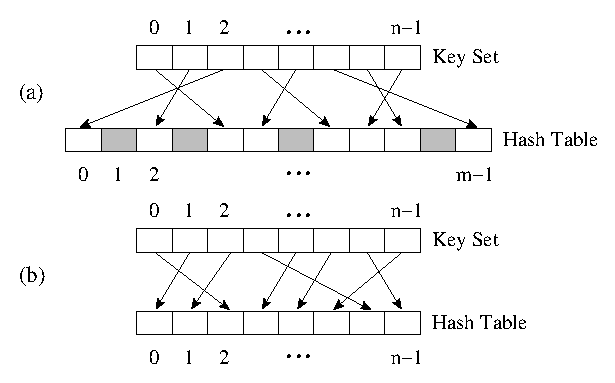
\includegraphics[width=0.45\textwidth, height=0.3\textheight]{figs/minimalperfecthash-ph-mph.ps}
% figure caption is below the figure
\caption{(a) Perfect hash function\quad  (b) Minimal perfect hash function}
\label{fig:minimalperfecthash-ph-mph}
\end{figure}

A aplicabilidade pr\'atica das FHPMs e consequentemente dos algoritmos utilizados para ger\'a-las est\'a diretamente relacionada com as seguintes m\'etricas:
\begin{enumerate}
\item Quantidade de tempo gasto para encontrar uma FHPM $h$.
\item Quantidade de mem\'oria exigida para encontrar $h$.  
\item Quantidade de tempo necess\'ario para avaliar ou computar $h$ para uma dada chave.
\item Quantidade de mem\'oria exigida para armazenar a descri\c{c}\~ao da fun\c{c}\~ao $h$.
\item Escalabilidade dos algoritmos com o crescimento de $S$. 
\end{enumerate}

Neste artigo apresentamos ...